% !TeX spellcheck = en_US
% !TeX root = ../MS_analysis_thesis.tex

\chapter{Description of Experiment}\label{chapter: Description of Experiment}
\section{Setup}
\lettrine[lhang = 0.4, findent=-60pt, lines=7]{\textbf{
		\initfamily \fontsize{40mm}{40mm} \selectfont O
		\normalfont}}{rikami}
is working on a project for MS patients, which includes the development of an app called `Mijn Kwik'.
In this project, daily data of MS patients will be gathered through wearables and a questionnaire app (\Cref{fig:app}).
%
\begin{figure}
	\centering
	\subfloat[Question about how your day was. It can be answered with \textit{good}, \textit{average} or \textit{bad}.]{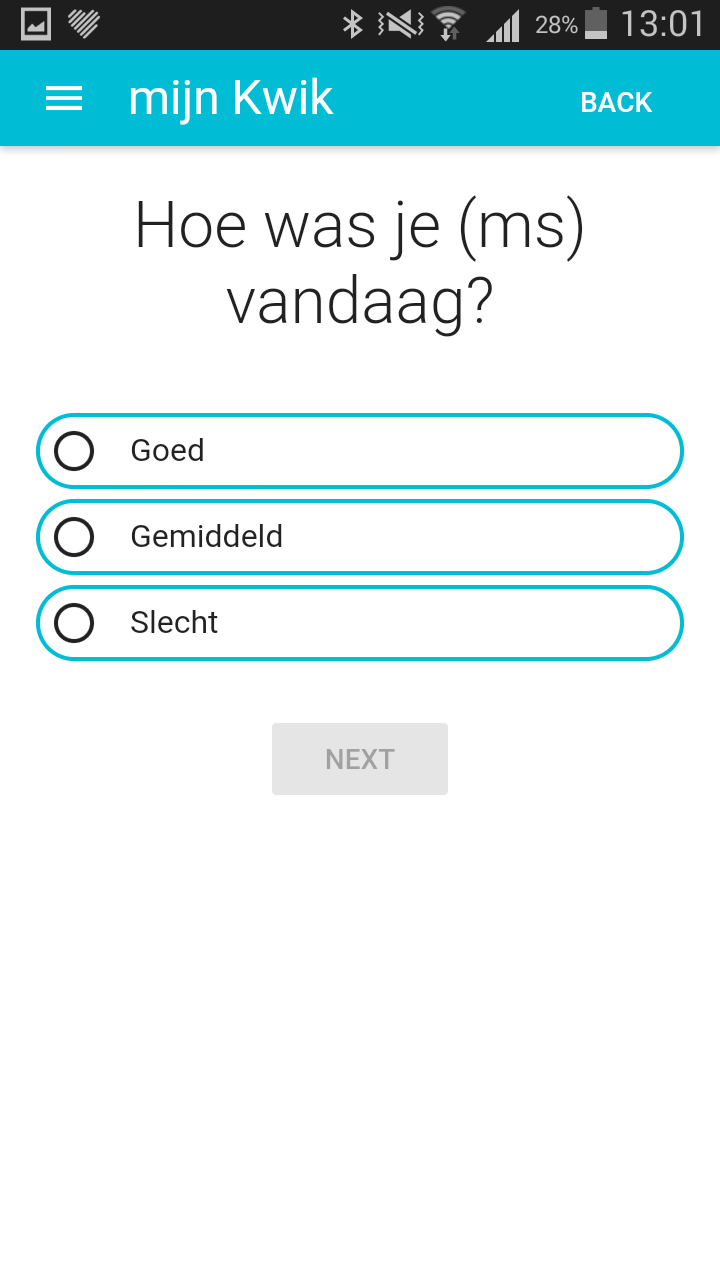
\includegraphics[scale=0.17]{DayIndicator}}
	\hspace{2cm}
	\subfloat[Question about your mood. The slider changes the happiness of the smiley, which represents your feeling today.]{\label{fig:app:mood}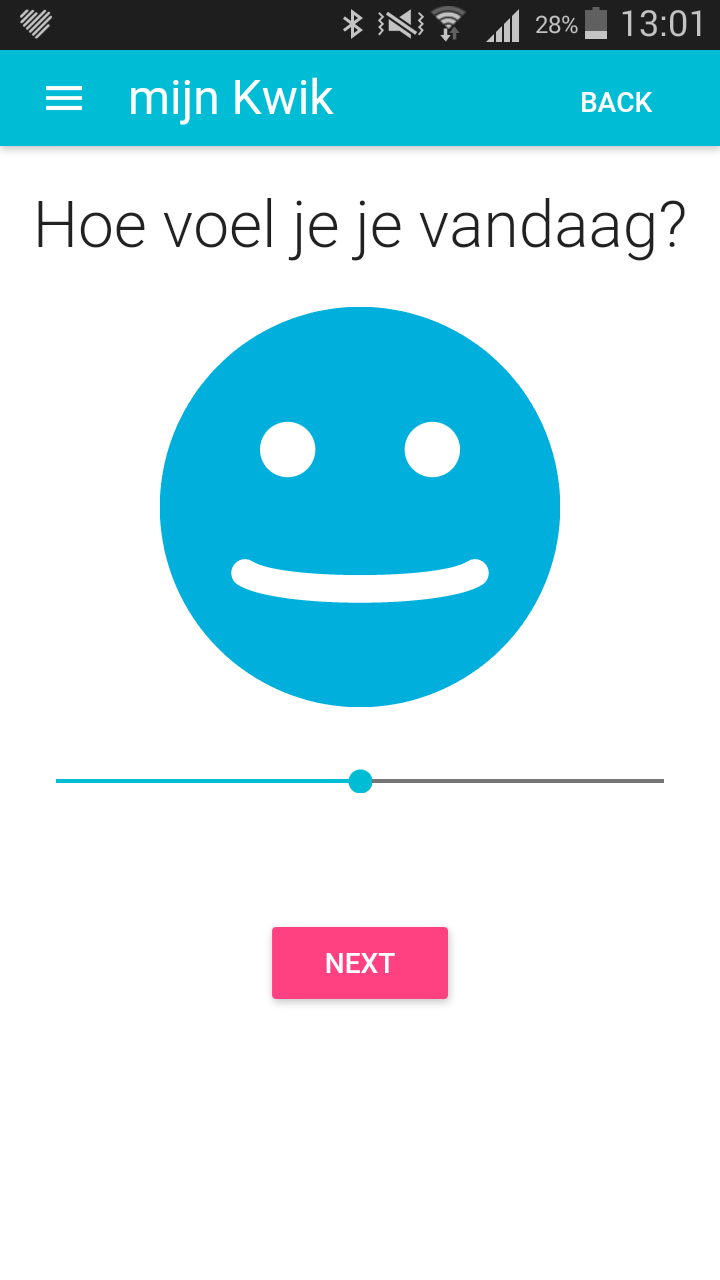
\includegraphics[scale=0.17]{MoodIndicator}}
	\vfill
	\subfloat[The walking test.]{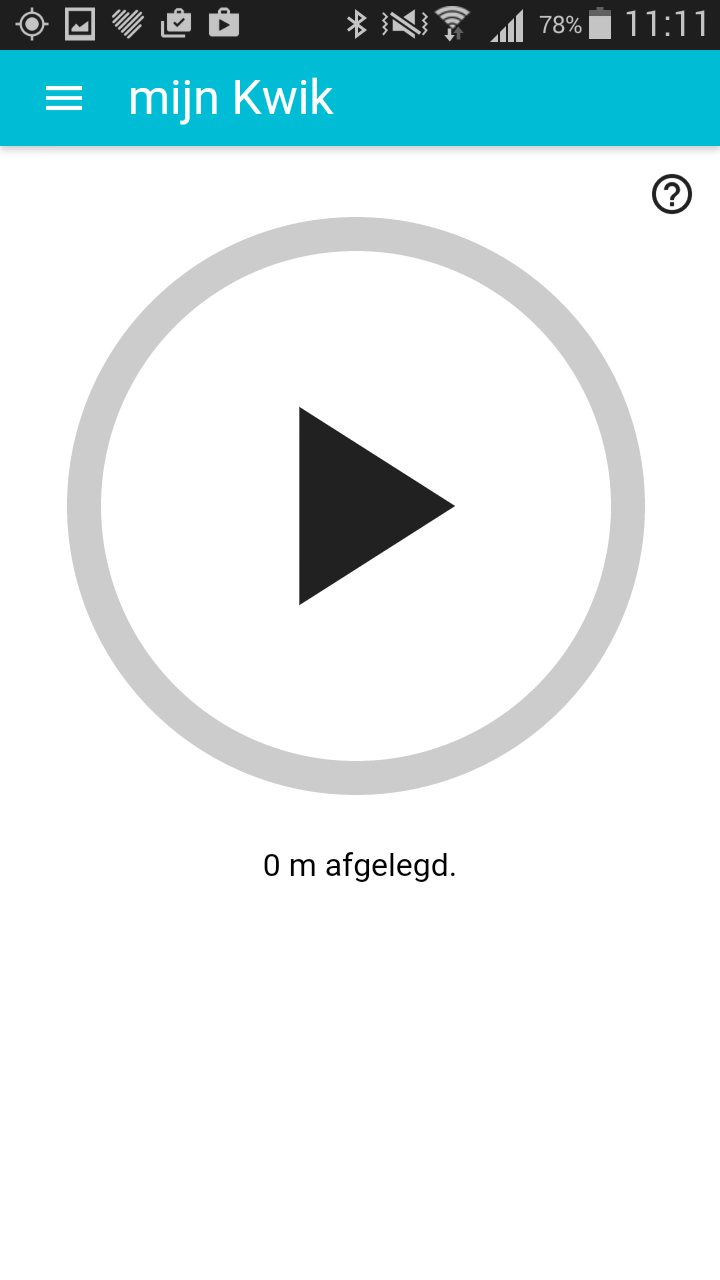
\includegraphics[scale=0.17]{WalkingTest}}
	\hspace{2cm}	
	\subfloat[For the variables \textit{energy}, \textit{mood}, \textit{stress}, \textit{memory}, \textit{concentration} and (not visible in the image) \textit{pain}, give an indication of the current value during this day using the corresponding sliders. ]{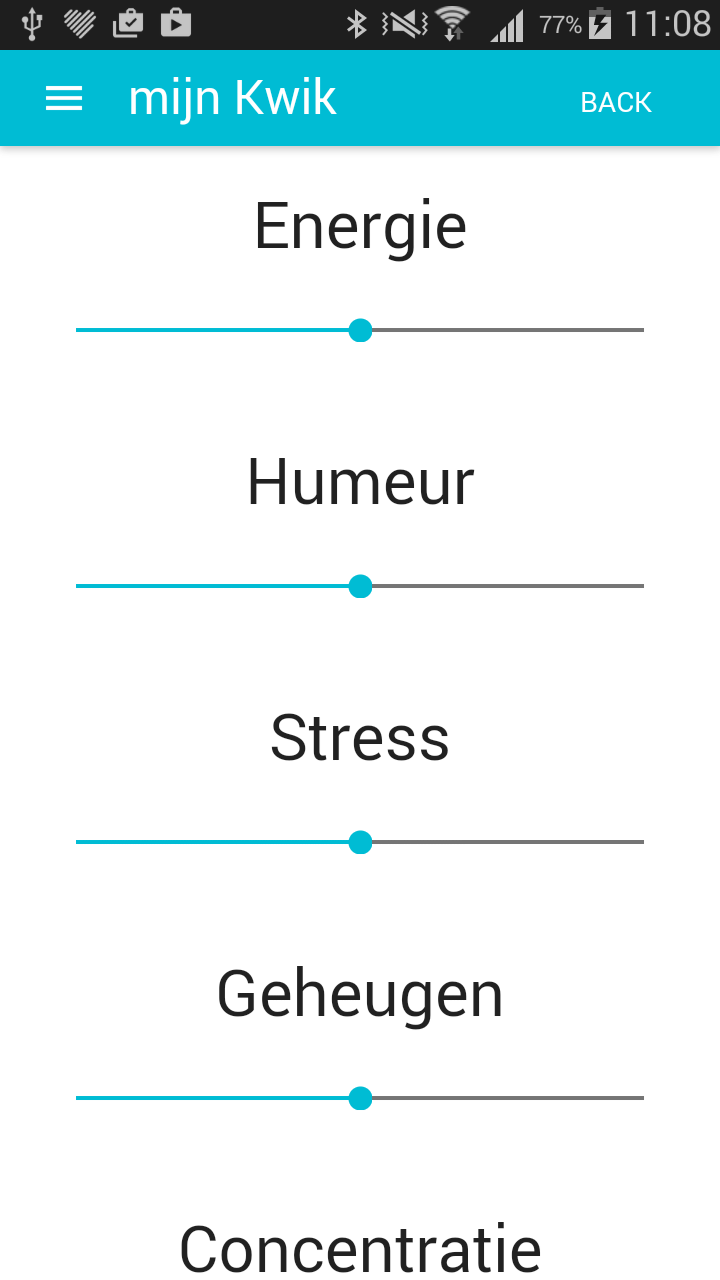
\includegraphics[scale=0.17]{VariablesIndicator}}
	
	\caption{Questions that must be answered and tasks that must be performed each day in the questionnaire app.}
	\label{fig:app}
\end{figure}
%
All of this data is gathered with the intention to predict good and bad days.
This study will be used to get more insight into the following aspects:
%
\begin{itemize}
	\item Stability of the application;
	\item Ease of use of the wearables and app for MS patients; 
	\item Problems with wearables during the experiment.
\end{itemize}
\parshape=0
%	   if a list has to be included in a paragraph starting with
%      a `lettrine', it is necessary to add the command |\parshape=0|
%      just after the end of the list (starting a new paragraph 
%      just before or just after the list works too)
%
We explained our plans at a meeting for MS patients organized by Orikami.
From all the people that attended the meeting, five patients volunteered to participate in the study.
A second meeting was organized to explain all the necessary details to the participants.
Each of the participants were given one of the following devices:
%
\begin{itemize}
	\item Basis Peak;
	\item Fitbit Charge HR;
	\item Microsoft Wristband 2.
\end{itemize}
\parshape=0
%
With our help, the participants were helped setting up the device and installing the corresponding mobile app on their phones.
Also an user agreement along with a privacy contract were handed out.
The latter had to be signed by each of the participants.
In this privacy contract, it is also stated that all of the gathered data will only be used for research purposes.

\section{Data storage} \label{section: Data storage}
Each of the activity trackers that are handed out to our participants will be linked to the Philips's ``Connect to Healthy''.
Through this service, the captured data will be synced to a database that can be used to access all of the data from the participants.
The data is stored in two databases, one containing the users, the measurement types and the actual measurements from the activity trackers. 
The other database contains the observations done through questions and the types of questions in the questionnaires.